\fenicschapter{Quadrature representation of finite element variational forms}
              {Quadrature representation of variational forms}
              {Kristian B. \O{}lgaard and Garth N. Wells}
              {oelgaard-2}

This chapter addresses the conventional run-time quadrature approach
for the numerical integration of local element tensors associated with
finite element variational forms, and in particular automated
optimizations that can be performed to reduce the number of floating
point operations. An alternative to the run-time quadrature approach
is the tensor representation presented in Chapter~\ref{chap:kirby-8}.
Both the quadrature and tensor approaches are implemented in \ffc{}
(see Chapter~\ref{chap:logg-1}).  In this chapter we discuss four
strategies for optimizing the quadrature representation for run-time
performance of the generated code and show that optimization
strategies lead to a dramatic improvement in run-time performance over
a naive implementation.  We also examine performance aspects of the
quadrature and tensor approaches for different equations, and this
will motivate the desirability of being able to choose between the two
representations.

\section{Standard quadrature representation}
\label{oelgaard-2:sec:standard_quadrature_representation}

To illustrate the standard quadrature representation \index{quadrature
representation} and optimizations implemented in \ffc{} we consider
the bilinear form for the weighted Laplace operator $-\nabla \cdot (w
\nabla u)$, where $u$ is the unknown and $w$ is a prescribed
coefficient.  The bilinear form of the variational problem for this
equation reads
%
\begin{equation}
  a\brac{u, v} = \int_{\Omega} w \nabla u \cdot \nabla v \dx.
  \label{oelgaard-2:eq:weightedlaplacian}
\end{equation}

The quadrature approach can deal with cases in which not all functions
come from a finite element space, using `quadrature functions' that
can be evaluated directly at quadrature points. The tensor
representation approach only supports cases in which all functions
come from a finite element space (using interpolation if necessary).
Therefore, to ensure a proper performance comparison between the
representations we assume that all functions in a form, including
coefficient functions, come from a finite element function space. In
the case of~\eqref{oelgaard-2:eq:weightedlaplacian}, all
functions will come from
%
\begin{equation}
  V_{h} = \bracc{v \in H^{1}\brac{\Omega}: \ v\vert_T \in P_{q}\brac{T}
    \foralls T \in \mathcal{T}},
  \label{oelgaard-2:eq:space_H1}
\end{equation}
%
where $P_{q}\brac{T}$ denotes the space of Lagrange polynomials of
degree $q$ on the element $T$ of the standard triangulation of
$\Omega$, which is denoted by~$\mathcal{T}$.  If we let
$\bracc{\phi^{T}_{i}}$ denote the local finite element basis that span
the discrete function space $V_{h}$ on $T$, the local element tensor
for an element $T$ can be computed as
%
\begin{equation}
  A_{T,i} = \int_{T} w \nabla \phi^{T}_{i_1} \cdot \nabla
  \phi^{T}_{i_2} \dx,
  \label{oelgaard-2:eq:localtensor}
\end{equation}
%
where $i = (i_{1}, i_{2})$.

The expression for the local element tensor
in~\eqref{oelgaard-2:eq:localtensor} can be expressed in \ufl{} (see
Chapter~\ref{chap:alnes-1}), from which \ffc{} generates an
intermediate representation of the form (see
Chapter~\ref{chap:logg-1}).  Assuming a standard affine mapping $F_T :
T_0 \rightarrow T$ from a reference element~$T_{0}$ to a given element
$T \in \mathcal{T}$, this intermediate representation reads
%
\begin{equation}
  A_{T,i}
  =
  \sum_{q=1}^{N}
  \sum_{\alpha_{3}=1}^n
  \Phi_{\alpha_{3}}(X^q)
  w_{\alpha_{3}}
  \sum_{\beta=1}^d
  \sum_{\alpha_1=1}^d
  \frac{\partial X_{\alpha_1}}{\partial x_{\beta}}
  \frac{\partial \Phi_{i_1}(X^q)}{\partial X_{\alpha_1}}
  \sum_{\alpha_2=1}^d
  \frac{\partial X_{\alpha_2}}{\partial x_{\beta}}
  \frac{\partial \Phi_{i_2}(X^q)}{\partial X_{\alpha_2}}
  \det F_T'
  W^q,
\label{oelgaard-2:eq:weightedlaplacian_quadraturerepresentation}
\end{equation}
%
where a change of variables from the reference coordinates $X$ to the
real coordinates $x = F_T(X)$ has been used. In the above equation,
$N$ denotes the number of integration points, $d$ is the dimension of
$\Omega$, $n$ is the number of degrees of freedom for the local basis
of~$w$, $\Phi_{i}$ denotes basis functions on the reference element,
$\det F_T'$ is the determinant of the Jacobian, and $W^q$ is the
quadrature weight at integration point~$X^q$.  By default, \ffc{}
applies a quadrature scheme that will integrate the variational form
exactly.  It calls FIAT (see Chapter~\ref{chap:kirby-2}) to compute
the quadrature scheme.  FIAT supplies schemes that are based on the
Gauss--Legendre--Jacobi rule mapped onto simplices
(see~\citet{KarniadakisSherwin2005} for details of such schemes).

From the representation
in~\eqref{oelgaard-2:eq:weightedlaplacian_quadraturerepresentation},
code for computing entries of the local element tensor is generated by
\ffc{}. This code is shown in
Figure~\ref{oelgaard-2:fig:standard_code}.  Code generated for the
quadrature representation is structured in the following way.  First,
values of geometric quantities that depend on the current element $T$,
like the components of the inverse of the Jacobian matrix $\partial
X_{\alpha_1} / \partial x_{\beta}$ and $\partial X_{\alpha_2}
/ \partial x_{\beta}$, are computed and assigned to the variables like
\emp{K\_01} in the code (this code is not shown as it is not important
for understanding the nature of the quadrature representation).  Next,
values of basis functions and their derivatives at integration points
on the reference element, like $\Phi_{\alpha_{3}}(X^q)$ and $\partial
\Phi_{i_1}(X^q) / \partial X_{\alpha_1}$ are tabulated.  Finite
element basis functions are computed by FIAT.  Basis functions and
their derivatives on a reference element are independent of the
current element $T$ and are therefore tabulated at compile-time and
stored in the tables \emp{Psi\_w}, \emp{Psi\_vu\_D01} and
\emp{Psi\_vu\_D10} in Figure~\ref{oelgaard-2:fig:standard_code}.
After the tabulation of basis functions values, the loop over
integration points begins.  In the example we are considering linear
elements, and only one integration point is necessary for exact
integration. The loop over integration points has therefore been
omitted.  The first task inside a loop over integration points is to
compute the values of coefficients at the current integration point.
For the considered problem, this involves computing the value of the
coefficient $w$.  The code for evaluating \emp{F0} in
Figure~\ref{oelgaard-2:fig:standard_code} is an exact translation of
the representation $\sum_{\alpha_{3}=1}^n \Phi_{\alpha_{3}}(X^q)
w_{\alpha_{3}}$.  The last part of the code in
Figure~\ref{oelgaard-2:fig:standard_code} is the loop over the basis
function indices $i_{1}$ and $i_{2}$, where the contribution to each
entry in the local element tensor, $A_{T}$, from the current
integration point is added.
To generate code using the quadrature representation the \ffc{}
command-line option \emp{-r quadrature} should be used.
%
\begin{figure}
\begin{c++}
virtual void tabulate_tensor(double* A,
                             const double * const * w,
                             const ufc::cell& c) const
{
  ...
  // Quadrature weight.
  static const double W1 = 0.5;

  // Tabulated basis functions at quadrature points.
  static const double Psi_w[1][3] = \
  {{0.33333333333333, 0.33333333333333, 0.33333333333333}};
  static const double Psi_vu_D01[1][3] = \
  {{-1.0, 0.0, 1.0}};
  static const double Psi_vu_D10[1][3] = \
  {{-1.0, 1.0, 0.0}};

  // Compute coefficient value.
  double F0 = 0.0;
  for (unsigned int r = 0; r < 3; r++)
    F0 += Psi_w[0][r]*w[0][r];

  // Loop basis functions.
  for (unsigned int j = 0; j < 3; j++)
  {
    for (unsigned int k = 0; k < 3; k++)
    {
      A[j*3 + k] +=\
      ((K_00*Psi_vu_D10[0][j] + K_10*Psi_vu_D01[0][j])*\
       (K_00*Psi_vu_D10[0][k] + K_10*Psi_vu_D01[0][k]) +\
       (K_01*Psi_vu_D10[0][j] + K_11*Psi_vu_D01[0][j])*\
       (K_01*Psi_vu_D10[0][k] + K_11*Psi_vu_D01[0][k])\
      )*F0*W1*det;
    }
  }
}
\end{c++}
\caption{Part of the generated code for the bilinear form associated
  with the weighted Laplacian using linear elements in two
  dimensions. The variables like \emp{K\_00} are components of the
  inverse of the Jacobian matrix and \emp{det} is the determinant of the
  Jacobian. The code to compute these variables is not shown. \emp{A}
  holds the values of the local element tensor and \emp{w} contains
  nodal values of the weighting function~$w$.}
\label{oelgaard-2:fig:standard_code}
\end{figure}


\section{Quadrature optimizations}
\label{oelgaard-2:sec:quadrature_optimizations}
\index{quadrature optimizations}

We now address optimizations for improving the run-time performance of
the generated code.  The underlying philosophy of the optimization
strategies implemented in \ffc{} is to manipulate the representation
in such a way that the number of operations to compute the local
element tensor decreases.  Each strategy described in the following
sections, with the exception of eliminating operations on zero terms,
share some common features which can be categorized as:

\begin{description}
\item[Loop invariant code motion] In short, this procedure seeks to
identify terms that are independent of one or more of the summation
indices and to move them outside the loop over those particular
indices.  For instance, in~\eqref{oelgaard-2:eq:%
weightedlaplacian_quadraturerepresentation} the terms regarding the
coefficient $w$, the quadrature weight $W^q$ and the determinant $\det
F_T'$ are all independent of the basis function indices $i_1$ and
$i_2$ and therefore only need to be computed once for each integration
point.  A generic discussion of this technique, which is also known as
`loop hoisting', can be found in~\citet{AhoSethiUllman1986}.
\index{loop hoisting}

\item[Reuse common terms] Terms that appear multiple times in an
  expression can be identified, computed once, stored as temporary
  values and then reused in all occurrences in the expression.  This can
  have a great impact on the operation count since the expression to
  compute an entry in $A_T$ is located inside loops over the basis
  function indices as shown in the code for the standard quadrature
  representation in Figure~\ref{oelgaard-2:fig:standard_code}.
\end{description}

To switch on optimization the command-line option \emp{-O} should be
used in addition to any of the \ffc{} optimization options presented
in the following sections.

\subsection{Eliminate operations on zeros}
\label{oelgaard-2:sec:eliminate_zeros}

Some basis functions and derivatives of basis functions may be
zero-valued at all integration points for a particular problem.  Since
these values are tabulated at compile-time, the columns containing
nonzero values can be identified.  This enables a reduction in the
loop dimension for indices concerning these tables.  However, a
consequence of reducing the tables is that a mapping of indices must
be created in order to access values correctly.  The mapping results
in memory not being accessed contiguously at run-time and can lead to a
decrease in run-time performance.

This optimization is switched on by using the command-line option
\emp{-f eliminate\_zeros}. Code for the weighted Laplace equation
generated with this option is shown in
Figure~\ref{oelgaard-2:fig:O_zeros_code}. For brevity, only code
different from that in Figure~\ref{oelgaard-2:fig:standard_code} has
been included.

\begin{figure}
\begin{c++}
// Tabulated basis functions.
static const double Psi_vu[1][2] = {{-1.0, 1.0}};

// Arrays of nonzero columns.
static const unsigned int nzc0[2] = {0, 2};
static const unsigned int nzc1[2] = {0, 1};

// Loop basis functions.
for (unsigned int j = 0; j < 2; j++)
{
 for (unsigned int k = 0; k < 2; k++)
 {
  A[nzc0[j]*3 + nzc0[k]] +=\
   (K_10*Psi_vu[0][j]*K_10*Psi_vu[0][k] +\
    K_11*Psi_vu[0][j]*K_11*Psi_vu[0][k])*F0*W1*det;
  A[nzc0[j]*3 + nzc1[k]] +=\
   (K_11*Psi_vu[0][j]*K_01*Psi_vu[0][k] +\
    K_10*Psi_vu[0][j]*K_00*Psi_vu[0][k])*F0*W1*det;
  A[nzc1[j]*3 + nzc0[k]] +=\
   (K_00*Psi_vu[0][j]*K_10*Psi_vu[0][k] +\
    K_01*Psi_vu[0][j]*K_11*Psi_vu[0][k])*F0*W1*det;
  A[nzc1[j]*3 + nzc1[k]] +=\
   (K_01*Psi_vu[0][j]*K_01*Psi_vu[0][k] +\
    K_00*Psi_vu[0][j]*K_00*Psi_vu[0][k])*F0*W1*det;
 }
}
\end{c++}
\caption{Part of the generated code for the weighted Laplacian using
  linear elements in two dimensions with optimization option \emp{-f
    eliminate\_zeros}.  The arrays \emp{nzc0} and \emp{nzc1} contain the
  nonzero column indices for the mapping of values.  Note how
  eliminating zeros makes it possible to replace the two tables with
  derivatives of basis functions \emp{Psi\_vu\_D01} and
  \emp{Psi\_vu\_D10} from Figure~\ref{oelgaard-2:fig:standard_code} with
  one table (\emp{Psi\_vu}).}
\label{oelgaard-2:fig:O_zeros_code}
\end{figure}

Although the elimination of zeros has lead to a decrease of the loop
dimension for the loops involving the indices \emp{j} and \emp{k} from
three to two, the number of operations has increased.  The reason is
that the mapping causes four entries to be computed at the same time
inside the loop, and the code to compute each entry has not been
reduced significantly if compared to the code in
Figure~\ref{oelgaard-2:fig:standard_code}.  In fact, using this
optimization strategy by itself is usually not recommended, but in
combination with the strategies outlined in the following sections it
can improve run-time performance significantly.  This effect is
particularly pronounced when forms contain mixed elements in which
many of the values in the basis function tables are zero.  Another
reason for being careful when applying this strategy is that the
increase in the number of terms might prevent \ffc{} compilation due
to hardware limitations.

\subsection{Simplify expressions}
\label{oelgaard-2:sec:simplify_expressions}

The expressions to evaluate an entry in the local element tensor can
become very complex. Since such expressions are typically located
inside loops, a reduction in complexity can reduce the total operation
count significantly.  The approach can be illustrated by the
expression $x (y + z) + 2 x y$, which after expansion of the first
term, grouping common terms and simplification can be reduced to $x (3
y + z)$, which involves a reduction from five to three operations.  An
additional benefit of this strategy is that the expansion of
expressions, which take place before the simplification, will
typically allow more terms to be precomputed and hoisted outside
loops, as explained in the beginning of this section.  For the
weighted Laplace equation, the terms
%
\begin{equation}
  \sum_{\beta=1}^d
  \sum_{\alpha_1=1}^d
    \frac{\partial X_{\alpha_1}}{\partial x_{\beta}}
    \frac{\partial \Phi_{i_1}(X^q)}{\partial X_{\alpha_1}}
  \sum_{\alpha_2=1}^d
    \frac{\partial X_{\alpha_2}}{\partial x_{\beta}}
    \frac{\partial \Phi_{i_2}(X^q)}{\partial X_{\alpha_2}}
\end{equation}
%
will be expanded into
%
\begin{equation}
  \sum_{\beta=1}^d
  \sum_{\alpha_1=1}^d
  \sum_{\alpha_2=1}^d
  \frac{\partial X_{\alpha_1}}{\partial x_{\beta}}
  \frac{\partial X_{\alpha_2}}{\partial x_{\beta}}
  \frac{\partial \Phi_{i_1}(X^q)}{\partial X_{\alpha_1}}
  \frac{\partial \Phi_{i_2}(X^q)}{\partial X_{\alpha_2}},
\end{equation}
%
where $\brac{\partial X_{\alpha_1} / \partial x_{\beta}}
\brac{\partial X_{\alpha_2} / \partial x_{\beta}}$ is independent of
the indices $i_1$ and $i_2$ and can therefore be moved outside these
loops.

The \ffc{} command-line option \emp{-f simplify\_expressions} should
be used to generate code with this optimization enabled.  Code
generated by this option for the representation
in~\eqref{oelgaard-2:eq:weightedlaplacian_quadraturerepresentation} is
presented in Figure~\ref{oelgaard-2:fig:O_simplify_code}, where again
only code different from that in
Figure~\ref{oelgaard-2:fig:standard_code} has been included.

\begin{figure}
\begin{c++}
// Geometry constants.
double G[3];
G[0] = W1*det*(K_00*K_00 + K_01*K_01);
G[1] = W1*det*(K_00*K_10 + K_01*K_11);
G[2] = W1*det*(K_10*K_10 + K_11*K_11);

// Integration point constants.
double I[3];
I[0] = F0*G[0];
I[1] = F0*G[1];
I[2] = F0*G[2];

// Loop basis functions.
for (unsigned int j = 0; j < 3; j++)
{
 for (unsigned int k = 0; k < 3; k++)
 {
  A[j*3 + k] += \
    (Psi_vu_D10[0][j]*Psi_vu_D10[0][k]*I[0] +\
     Psi_vu_D10[0][j]*Psi_vu_D01[0][k]*I[1] +\
     Psi_vu_D01[0][j]*Psi_vu_D10[0][k]*I[1] +\
     Psi_vu_D01[0][j]*Psi_vu_D01[0][k]*I[2]);
 }
}
\end{c++}
\caption{Part of the generated code for the weighted Laplacian using
  linear elements in two dimensions with optimization option \emp{-f
    simplify\_expressions}.}
\label{oelgaard-2:fig:O_simplify_code}
\end{figure}

Due to expansion of the expression, many terms related to the geometry
have been moved outside of the loops over the basis function indices
\emp{j} and \emp{k} and stored in the array~\emp{G}.  Also, note how
the expressions to compute the values in \emp{G} have been simplified
by moving the variables \emp{det} and \emp{W1} outside the
parentheses.  Similarly, terms that depend only on the integration
point are hoisted and stored in the array~\emp{I}.  The number of
operations has decreased compared to the code in
Figure~\ref{oelgaard-2:fig:standard_code} for the standard quadrature
representation. An improvement in run-time performance can therefore be
expected.

The optimization described above is the most expensive of the
quadrature optimizations to perform in terms of \ffc{} code generation
time and memory consumption as it involves creating new terms when
expanding the expressions.  The
procedure does not scale well for complex expressions, but it is in
many cases the most effective approach in terms of reducing the number
of operations.  This particular optimization strategy, in combination
with the elimination of zeros outlined in the previous section, was
the first to be implemented in \ffc{}.  It has been investigated and
compared to the tensor representation in~\citet{OelgaardWells2010}, to
which the reader is referred for further details.

\subsection{Precompute integration point constants}

The optimizations described in the previous section are performed at
the expense of increased code generation time.  In order to reduce the
generation time while achieving a reduction in the operation count,
another approach can be taken involving hoisting expressions that are
constant with respect to integration points without expanding the
expression first.

To generate code with this optimization the \ffc{} command-line option
\emp{-f precompute\_ip\_const} should be used.  Code generated by this
method for the representation
in~\eqref{oelgaard-2:eq:weightedlaplacian_quadraturerepresentation}
can be seen in Figure~\ref{oelgaard-2:fig:O_ip_code}.

\begin{figure}
\begin{c++}
// Geometry constants.
double G[1];
G[0] = W1*det;

// Integration point constants.
double I[1];
I[0] = F0*G[0];

// Loop basis functions.
for (unsigned int j = 0; j < 3; j++)
{
  for (unsigned int k = 0; k < 3; k++)
  {
    A[j*3 + k] +=\
    ((Psi_vu_D01[0][j]*K_10 + Psi_vu_D10[0][j]*K_00)*\
     (Psi_vu_D01[0][k]*K_10 + Psi_vu_D10[0][k]*K_00) +\
     (Psi_vu_D01[0][j]*K_11 + Psi_vu_D10[0][j]*K_01)*\
     (Psi_vu_D01[0][k]*K_11 + Psi_vu_D10[0][k]*K_01)
    )*I[0];
  }
}
\end{c++}
\caption{Part of the generated code for the weighted Laplacian using
  linear elements in two dimensions with optimization option \emp{-f
    precompute\_ip\_const}.}
\label{oelgaard-2:fig:O_ip_code}
\end{figure}

It is clear from the generated code that this strategy will not lead
to a significant reduction in the number of operations for this
particular form. However, for more complex forms, with many
coefficients, the number of terms that can be hoisted will increase
significantly, leading to improved run-time performance.

\subsection{Precompute basis constants}

This optimization strategy is an extension of the strategy described
in the previous section. In addition to hoisting terms related to the
geometry and the integration points, values that depends on the basis
indices are precomputed inside the loops.  This will result in a
reduction in operations for cases in which some terms appear
frequently inside the loop such that a given value can be reused once
computed.

To generate code with this optimization, the \ffc{}
command-line option \emp{-f precompute\_basis\_const} should
be used.  Code generated by this method for the representation
in~\eqref{oelgaard-2:eq:weightedlaplacian_quadraturerepresentation}
can be seen in Figure~\ref{oelgaard-2:fig:O_basis_code}, where only
code that differs from that in Figure~\ref{oelgaard-2:fig:O_ip_code}
has been included.  In this particular case, no additional reduction in
operations has been achieved, if compared to the previous method, since no
terms can be reused inside the loop over the indices \emp{j} and~\emp{k}.

\begin{figure}
\begin{c++}
for (unsigned int j = 0; j < 3; j++)
{
  for (unsigned int k = 0; k < 3; k++)
  {
    double B[16];
    B[0] = Psi_vu_D01[0][j]*K_10;
    B[1] = Psi_vu_D10[0][j]*K_00;
    B[2] = (B[0] + B[1]);
    B[3] = Psi_vu_D01[0][k]*K_10;
    B[4] = Psi_vu_D10[0][k]*K_00;
    B[5] = (B[3] + B[4]);
    B[6] = B[2]*B[5];
    B[7] = Psi_vu_D01[0][j]*K_11;
    B[8] = Psi_vu_D10[0][j]*K_01;
    B[9] = (B[7] + B[8]);
    B[10] = Psi_vu_D01[0][k]*K_11;
    B[11] = Psi_vu_D10[0][k]*K_01;
    B[12] = (B[10] + B[11]);
    B[13] = B[12]*B[9];
    B[14] = (B[13] + B[6]);
    B[15] = B[14]*I[0];
    A[j*3 + k] += B[15];
  }
}
\end{c++}
\caption{Part of the generated code for the weighted Laplacian using
  linear elements in two dimensions with optimization option \emp{-f
    precompute\_basis\_const}. The array \emp{B} contain precomputed
  values that depend on indices \emp{j} and \emp{k}.}
\label{oelgaard-2:fig:O_basis_code}
\end{figure}


\subsection{Future optimizations}

Preliminary investigations suggest that the performance of the
quadrature representation can be improved by applying two additional
optimizations.  Looking at the code in
Figure~\ref{oelgaard-2:fig:O_basis_code}, we see that about half of
the temporary values in the array \emp{B} only depend on the loop
index \emp{j}, and they can therefore be hoisted, as we have done for
other terms in previous sections.  Another approach is to unroll the
loops with respect to \emp{j} and \emp{k} in the generated code.  This
will lead to a dramatic increase in the number of values that can be
reused, and the approach can be readily combined with all of the other
optimization strategies. However, the total number of temporary values
will also increase. Therefore, this optimization strategy might not be
feasible for all forms.

\ffc{} uses a Gauss--Legendre--Jacobi quadrature scheme mapped onto
simplices for the numerical integration of variational forms.  This
means that for exact integration of a second-order polynomial, \ffc{}
will use two quadrature points in each spatial direction that is, $2^3
= 8$ points per cell in three dimensions.  A further optimization of
the quadrature representation can thus be achieved by implementing
more efficient quadrature schemes for simplices since a reduction in
the number of integration points will yield improved run-time
performance.  \ffc{} does, however, provide an option for a user to
specify the quadrature degree of a variational form thereby permitting
inexact quadrature.  To set the quadrature degree equal to one, the
command-line option \emp{-f quadrature\_degree=1} should be used.

\section{Performance comparisons}

In this section we investigate the impact of the optimization
strategies outlined in the previous section on the run-time
performance. The point is not to present a rigorous analysis of the
optimizations, but to provide indications as to when the different
strategies will be most effective. We also compare the run-time
performance of quadrature representation to the tensor representation,
which is described in Chapter~\ref{chap:kirby-8}, to illustrate the
strengths and weaknesses of the two approaches.

\subsection{Performance of quadrature optimizations}
\label{oelgaard-2:sec:quad_performance}

The performance of the quadrature optimizations will be investigated
using two forms, namely the bilinear form for the weighted Laplace
equation~\eqref{oelgaard-2:eq:weightedlaplacian} and the bilinear form
for the hyperelasticity model presented in Chapter~\ref{chap:alnes-1},
equation~\eqref{alnes-1:eq:hypdefa}.  In both cases quadratic Lagrange
finite elements will be used.

All tests were performed on an Intel Pentium M CPU at 1.7GHz with
1.0GB of RAM running Ubuntu 10.04 with Linux kernel 2.6.32.  We used
Python version 2.6.5 and NumPy version 1.3.0 (both pertinent to
\ffc{}), and g++ version 4.4.3 to compile the \ufc{} version 1.4
compliant C++ code.

The two forms are compiled with the different \ffc{} optimizations,
and the number of floating point operations (flops) \index{flops} to
compute the local element tensor is determined.  We define the number
of flops as the sum of all appearances of the operators `\emp{+}' and
`\emp{*}' in the code.  The ratio between the number of flops of the
current \ffc{} optimization and the standard quadrature
representation, `$o/q$' is also computed.  The generated code is then
compiled with g++ using four different optimization options and the
time needed to compute the element tensor $N$ times is measured.  In
the following, we will use \emp{-zeros} as shorthand for the \emp{-f
eliminate\_zeros} option, \emp{-simplify} as shorthand for the \emp{-f
simplify\_expressions} option, \emp{-ip} as shorthand for the \emp{-f
precompute\_ip\_const} option and \emp{-basis} as shorthand for the
\emp{-f precompute\_basis\_const} option.

The operation counts for the weighted Laplace equation with different
\ffc{} optimizations can be seen in
Table~\ref{oelgaard-2:tab:laplace_stats_1}, while
Figure~\ref{oelgaard-2:fig:laplace_stats_2} shows the run-time
performance for different compiler options for $N = 1 \times 10^7$.
The \ffc{} compiler options can be seen on the $x$-axis in the figure
and the four g++ compiler options are shown with different colors.

\begin{table}
  \caption{Operation counts for the weighted Laplace equation.}
  \label{oelgaard-2:tab:laplace_stats_1}
  \centering
  \begin{tabular}{lrr}
    \toprule
    \multicolumn{1}{c}{\ffc{}}       &\multicolumn{2}{c}{}       \\
    \multicolumn{1}{c}{optimization} & flops & o/q   \\
    \midrule
    \emp{None}                       &  6264 &  1.00 \\
    \emp{-zeros}                     & 10008 &  1.60 \\
    \emp{-simplify}                  &  4062 &  0.65 \\
    \emp{-simplify -zeros}           &  2874 &  0.45 \\
    \emp{-ip}                        &  5634 &  0.90 \\
    \emp{-ip -zeros}                 &  6432 &  1.03 \\
    \emp{-basis}                     &  5634 &  0.90 \\
    \emp{-basis -zeros}              &  5532 &  0.88 \\
    \bottomrule
  \end{tabular}
\end{table}

\begin{figure}
  \ffigbox{\caption{Run-Time performance for the weighted Laplace
      equation for different compiler options.  The $x$-axis shows the
      \ffc{} compiler options, and the colors denote the g++ compiler
      options.}\label{oelgaard-2:fig:laplace_stats_2}}
          {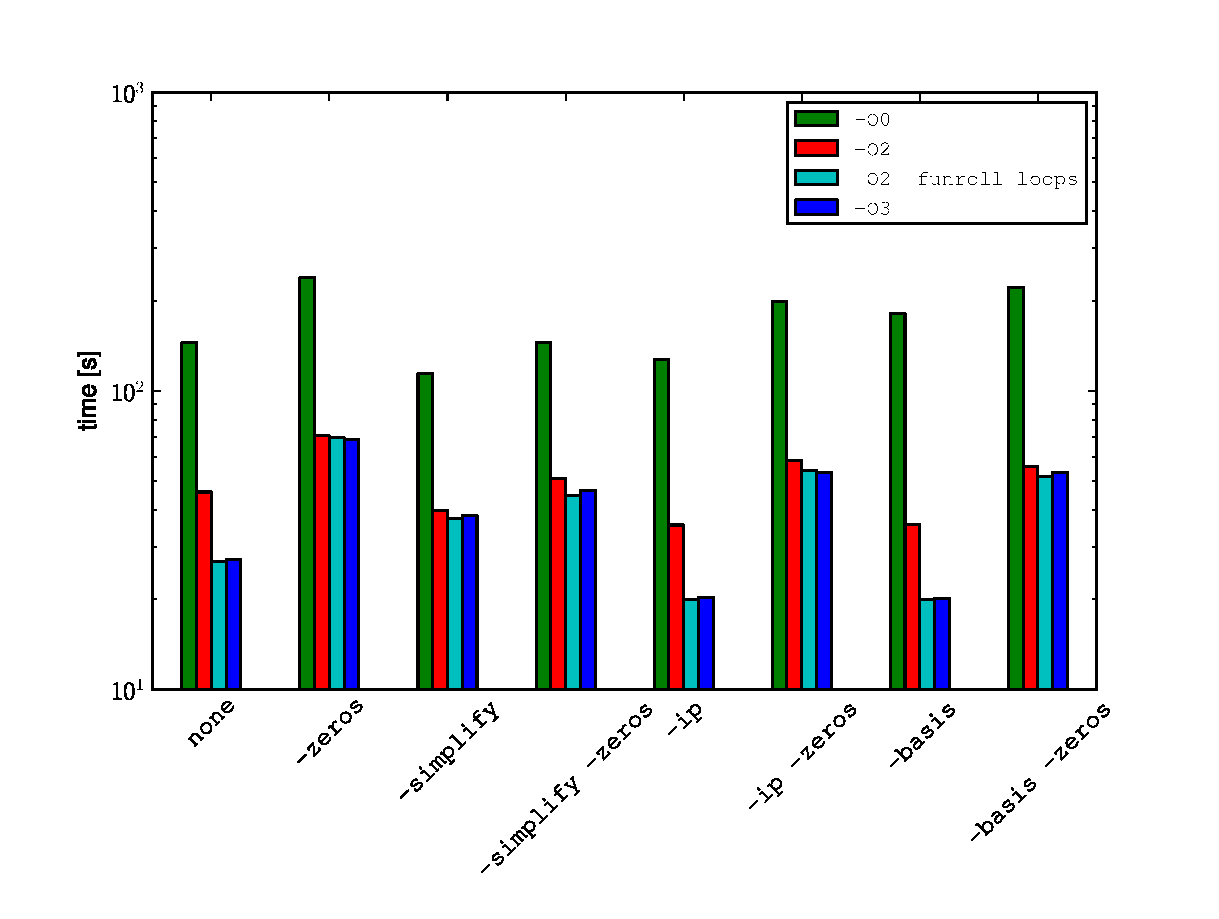
\includegraphics[width=\fullfig]{chapters/oelgaard-2/pdf/runtime_laplace.pdf}}
\end{figure}

The \ffc{} and g++ compile-times were less than one second for all
optimization options.  It is clear from
Figure~\ref{oelgaard-2:fig:laplace_stats_2} that run-time performance
is greatly influenced by the g++ optimizations.  Compared to the case
where no g++ optimizations are used (the \emp{-O0} flag), the run-time
for the standard quadrature code improves by a factor of 3.15 when
using the \emp{-O2} option and 5.40 when using the \emp{-O2
-funroll-loops} option.  The \emp{-O3} option does not appear to
improve the run-time noticeably beyond the improvement observed for the
\emp{-O2 -funroll-loops} option.  Using the \ffc{} optimization option
\emp{-zeros} alone for this form does not improve run-time performance.
In fact, using this option in combination with any of the other
optimization options increases the run-time, even when combining with
the option \emp{-simplify}, which has a significant lower operation
count compared to the standard quadrature representation.  A curious
point to note is that without g++ optimization there is a significant
difference in run-time for the \emp{-ip} and \emp{-basis} options, even
though they involve the same number of flops.  When g++ optimizations
are switched on, this difference is eliminated completely and the
run-time for the two \ffc{} optimizations are identical.  This suggests
that it is not possible to predict run-time performance from the
operation count alone since the type of \ffc{} optimization must be
taken into account as well as the intended use of g++ compiler
options.  The optimal combination of optimizations for this form is
\ffc{} option \emp{-ip} or \emp{-basis} combined with g++ option
\emp{-O2 -funroll-loops}, in which case the run-time has improved by a
factor of 7.23 compared to standard quadrature code with no g++
optimizations.

The operation counts and \ffc{} compile-time for the bilinear form for
hyperelasticity with different \ffc{} optimizations are presented in
Table~\ref{oelgaard-2:tab:hyper_stats_1}, while
Figure~\ref{oelgaard-2:fig:hyper_stats_2} shows the run-time
performance for different compiler options for $N = 1 \times 10^4$.
%
\begin{table}
  \caption{\ffc{} compile-times and operation counts for the
    hyperelasticity example.}
  \label{oelgaard-2:tab:hyper_stats_1}
  \centering
  \begin{tabular}{lrrrr}
    \toprule
    \multicolumn{1}{c}{\ffc{}}       & \multicolumn{2}{c}{\ffc{} time} & \multicolumn{2}{c}{} \\
    \multicolumn{1}{c}{optimization} & {\scriptsize [s]} & o/q         & flops     & o/q      \\
    \midrule
    \emp{None}                       &  8.1              & 1.00        & 136531980 & 1.000 \\
    \emp{-zeros}                     &  8.3              & 1.02        &  60586218 & 0.444 \\
    \emp{-simplify}                  & 22.3              & 2.75        &   5950646 & 0.044 \\
    \emp{-simplify -zeros}           & 21.2              & 2.62        &    356084 & 0.003 \\
    \emp{-ip}                        & 15.2              & 1.88        &  90146710 & 0.660 \\
    \emp{-ip -zeros}                 & 17.9              & 2.21        &  14797360 & 0.108 \\
    \emp{-basis}                     & 15.2              & 1.88        &   7429510 & 0.054 \\
    \emp{-basis -zeros}              & 17.8              & 2.20        &   1973521 & 0.014 \\
    \bottomrule
  \end{tabular}
\end{table}
%
\begin{figure}
  \ffigbox{\caption{Run-Time performance for the hyperelasticity
      example for different compiler options. The $x$-axis shows the
      \ffc{} compiler options, and the colors denote the g++ compiler
      options.}\label{oelgaard-2:fig:hyper_stats_2}}
          {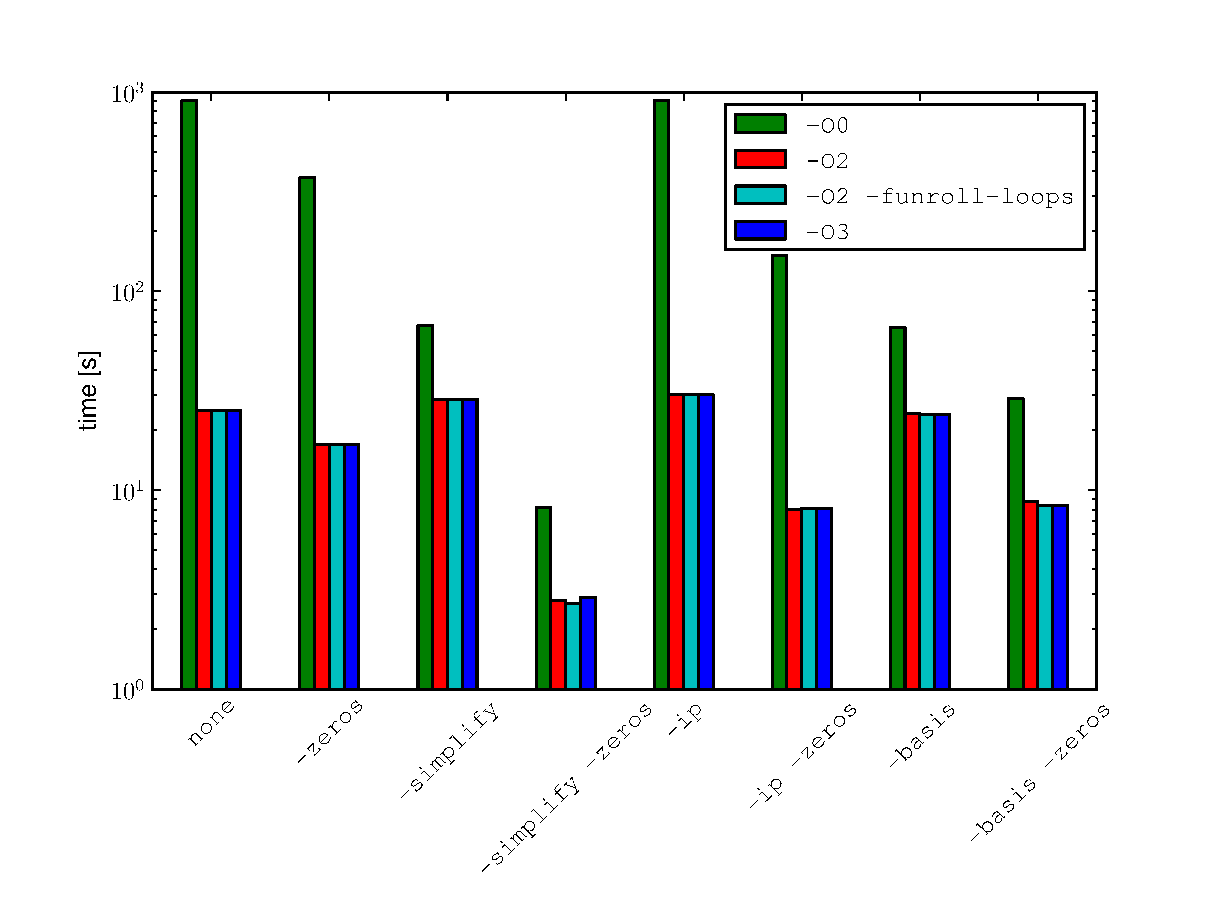
\includegraphics[width=\fullfig]{chapters/oelgaard-2/pdf/runtime_hyperelasticity.pdf}}
\end{figure}
%
Comparing the number of flops involved to compute the element tensor
to the weighted Laplace example, it is clear that this problem is
considerably more complex.  The \ffc{} compile-times in
Table~\ref{oelgaard-2:tab:hyper_stats_1} show that the \emp{-simplify}
optimization, as anticipated, is the most expensive to perform.  The
g++ compile-times for all test cases were in the range two to six
seconds for all optimization options.  A point to note is that the
scope for reducing the flop count is considerably greater for this
problem than for the weighted Laplace problem, with a difference in
the number of flops spanning several orders of magnitude between the
different \ffc{} optimizations.  This compares to a difference in
flops of roughly a factor two between the non-optimized and the most
effective optimization strategy for the weighted Laplace problem.  In
the case where no g++ optimization is used the run-time performance
for the hyperelastic problem can be directly related to the number of
floating point operations.  When the g++ optimization \emp{-O2} is
switched on, this effect becomes less pronounced.  Another point to
note, in connection with the g++ optimizations, is that switching on
additional optimizations beyond \emp{-O2} does not seem to provide any
further improvements in run-time.  For the hyperelasticity example,
the option \emp{-zeros} has a positive effect on the performance, not
only when used alone but in particular when combined with the other
\ffc{} optimizations.  This is in contrast with the weighted Laplace
equation. The reason is that the test and trial functions are vector
valued rather than scalar valued, which allows more zeros to be
eliminated.  Finally, it is noted that the \emp{-simplify} option
performs particularly well for this example compared to the weighted
Laplace problem.  The reason is that the nature of the hyperelasticity
form results in a relatively complex expression to compute the entries
in the local element tensor.  However, this expression only consists
of a few different variables (components of the inverse of the
Jacobian and basis function values) which makes the \emp{-simplify}
option very efficient since many terms are common and can be
precomputed and hoisted.  For the hyperelasticity form, the optimal
combination of optimizations is \ffc{} option \emp{-simplify -zeros}
and g++ option \emp{-O2 -funroll-loops} which improves the run-time
performance of the code by a factor of 3149 when compared to the case
where no optimization is used by either \ffc{} or~g++.

For the considered examples, it is clear that no single optimization
strategy is the best for all cases.  Furthermore, the generation phase
optimizations that one can best use depends on which optimizations are
performed by the g++ compiler.  It is also very likely that different
C++ compilers will give different results for the test cases presented
above.  The general recommendation for selecting the appropriate
optimization for production code will therefore be that the choice
should be based on a benchmark program for the specific problem.

\subsection{Relative performance of the quadrature and tensor
  representations}
\label{oelgaard-2:sec:performance_of_representations}

As demonstrated in the previous section, a given type of optimization
may be effective for one class of forms, and be less effective for
another class of forms.  Similarly, differences can be observed
between the quadrature and tensor representations for different
equations.  A detailed study on this issue was carried out
in~\citet{OelgaardWells2010}.  For convenience we reproduce here the
main conclusions along with
Table~\ref{oelgaard-2:tab:elasticity2D_complex_comparison}, which has
been reproduced from the paper.  The results shown in this section
pertain to an elasticity-like bilinear form in two dimensions that is
premultiplied by a number of scalar coefficients~$f_{i}$:
%
\begin{equation}
  a\brac{u, v} = \int_{\Omega} (f_0 f_1, \ldots, f_{n_f} )\ \nabla^s u
  : \nabla^s v \dx,
  \label{oelgaard-2:eq:elasticity_form}
\end{equation}
%
where $n_f$ is the number of premultiplying coefficients.
The test and trial functions are denoted by $v, u \in V_{h}$, with
%
\begin{equation}
  V_{h} = \bracc{v \in [H^{1}\brac{\Omega}]^2: \ v\vert_T \in
    [P_{q}\brac{T}]^2 \foralls T \in \mathcal{T}}
 \label{oelgaard-2:eq:elastictity_H1_vector_space}
\end{equation}
%
and the coefficient functions $f_{i} \in W_{h}$ with
%
\begin{equation}
  W_{h} = \bracc{f \in H^{1}\brac{\Omega}: \ f\vert_T \in
    P_{p}\brac{T} \foralls T \in \mathcal{T}},
 \label{oelgaard-2:eq:elasticity_H1_space}
\end{equation}
%
where $q$ and $p$ denote the polynomial order of the
Lagrange basis functions.  The number of coefficients and the
polynomial orders are varied and the number of flops needed to compute
the local element tensor is recorded for both tensor and quadrature
representations.  The results were obtained by using the optimization
options \emp{-f eliminate\_zeros -f simplify\_expressions} for the
quadrature representation.  In Table~\ref{oelgaard-2:tab:%
elasticity2D_complex_comparison} the flops for the tensor
representation is presented together with the ratio given by the flops
for quadrature representation divided by the flops for tensor
representation, denoted by $q/t$.  In terms of flops, a ratio $q/t >
1$ indicates that the tensor representation is more efficient while
$q/t < 1$ indicates that the quadrature representation is more
efficient.  It was found that when comparing the run-time performance
of the two representations for this problem that the number of flops
is a good indicator of performance.  However, as we have shown in the
previous section, the quadrature code with the lowest number of flops
does not always perform best for a given form. Furthermore, the
run-time performance even depends on which g++ options are used.  This
begs the question of whether or not it is possible to make a sound
selection between representations based only on an estimation of
flops, as suggested in~\citet{OelgaardWells2010}.

\begin{table}
  \caption{The number of operations and the ratio between number of
    operations for the two representations for the elasticity-like
    tensor in two dimensions as a function of different polynomial
    orders and numbers of functions (taken from
    \citet{OelgaardWells2010}.}
  \label{oelgaard-2:tab:elasticity2D_complex_comparison}
  \centering
  \small
  \begin{tabular}{lrrrrrr}
    \toprule
    \multicolumn{1}{c}{} & \multicolumn{2}{c}{$n_f = 1$} & \multicolumn{2}{c}{$n_f = 2$} & \multicolumn{2}{c}{$n_f = 3$}\\
    & flops & q/t          & flops & q/t          & flops & q/t\\
    \midrule
    $p = 1$, $q = 1$  &    888  &  0.34               &    3060 &  0.36               &   10224 & 0.11\\
    $p = 1$, $q = 2$  &   3564  &  1.42               &   11400 &  1.01               &   35748 & 0.33\\
    $p = 1$, $q = 3$  &  10988  &  3.23               &   34904 &  1.82               &  100388 & 0.63\\
    $p = 1$, $q = 4$  &  26232  &  5.77               &   82548 &  2.87               &  254304 & 0.93\\
    \midrule
    $p = 2$, $q = 1$  &    888  &  1.20               &    8220 &  0.31               &   54684 & 0.09\\
    $p = 2$, $q = 2$  &   7176  &  1.59               &   41712 &  0.49               &  284232 & 0.11\\
    $p = 2$, $q = 3$  &  22568  &  2.80               &  139472 &  0.71               &  856736 & 0.17\\
    $p = 2$, $q = 4$  &  54300  &  4.36               &  337692 &  1.01               & 2058876 & 0.23\\
    \midrule
    $p = 3$, $q = 1$  &   3044  &  0.36               &   30236 &  0.16               &  379964 & 0.02\\
    $p = 3$, $q = 2$  &  12488  &  0.92               &  126368 &  0.26               & 1370576 & 0.03\\
    $p = 3$, $q = 3$  &  36664  &  1.73               &  391552 &  0.37               & 4034704 & 0.05\\
    $p = 3$, $q = 4$  &  92828  &  2.55               &  950012 &  0.49               & 9566012 & 0.06\\
    \midrule
    $p = 4$, $q = 1$  &   3660  &  0.68               &   73236 &  0.11               & 1275624 & 0.01\\
    $p = 4$, $q = 2$  &  17652  &  1.16               &  296712 &  0.16               & 4628460 & 0.02\\
    $p = 4$, $q = 3$  &  57860  &  1.71               &  903752 &  0.22               &13716836 & 0.02\\
    $p = 4$, $q = 4$  & 138984  &  2.46               & 2133972 &  0.29               &32289984 & 0.03\\
    \bottomrule
  \end{tabular}
\end{table}

Nevertheless, some general trends can still be read from the table.
Increasing the number of coefficient functions $n_f$ in the form
clearly works in favor of quadrature representation.  For $n_{f}=3$
the quadrature representation can be expected to perform best for all
values of $q$ and~$p$.  Increasing the polynomial order of
the coefficients, $p$, also works in favor of quadrature representation
although the effect is less pronounced compared to the effect of
increasing the number of coefficients.  The tensor representation
appears to perform better when the polynomial order of the test and
trial functions, $q$, is increased although the effect is most
pronounced when the number of coefficients is low.

\section{Automatic selection of representation}

We have illustrated how the run-time performance of the generated code
for variational forms can be improved by using various optimization
options for the \ffc{} and g++ compilers, and by changing the
representation of the form.  Choosing the combination of form
representation and optimization options that leads to optimal
performance will inevitably require a benchmark study of the specific
problem.  However, very often many variational forms of varying
complexity are needed to solve more complex problems. Setting up
benchmarks for all of them is cumbersome and time consuming.
Additionally, during the model development stage run-time performance
is of minor importance compared to rapid prototyping of variational
forms as long as the generated code performs reasonably well.

The default behavior of \ffc{} is, therefore, to automatically
determine which form representation should be used based on a measure
for the cost of using the tensor representation.  In short, the cost
is simply computed as the maximum value of the sum of the number of
coefficients and derivatives present in the monomials representing the
form.  If this cost is larger than a specified threshold, currently
set to three, the quadrature representation is selected.  Recall from
Table~\ref{oelgaard-2:tab:elasticity2D_complex_comparison} that when
$n_f=3$ the flops for quadrature representation was significantly
lower for virtually all the test cases.  Although this approach may
seem \emph{ad hoc}, it will work well for those situations where the
difference in run-time performance is significant.  It is important to
remember that the generated code is only concerned with the evaluation
of the local element tensor and that the time needed to insert the
values into a sparse matrix and to solve the system of equations will
reduce any difference, particularly for simple forms.  Therefore,
making a correct choice of representation is less important for forms
where the difference in run-time performance is small.  A future
improvement could be to devise a strategy for also letting the system
select the optimization strategy for the quadrature representation
automatically.
